\section{Modello Computazionale}
Il modello computazionale consiste in un programma di simulazione di tipo
next-event che impiega il metodo ``batch means'' per il calcolo di tutte le
metriche di interesse. 
A questo livello di astrazione del sistema si passa ad implementare tutto ciò
che è stato definito formalmente nel modello di specifica, in particolare in
questa sezione verranno descritte le strutture dati impiegate per la
rappresentazione delle variabili, le funzioni ed i costrutti che realizzano la
logica del sistema, come vengono generati i dati di input ed infine le
metodologie con cui vengono collezionati ed elaborati i dati di output.
%
%
\subsection{Strutture dati}
In primo luogo, vengono definite le strutture dati riguardanti la lista degli
eventi possibili ed il clock che regola il tempo di simulazione, successivamente
quelle che contegono i dati di output ed infine la struttura dati relativa alla
principale entità manipolata nel sistema: il job.
%
\subsubsection{Eventi e clock virtuale}
Ad ogni istante la lista di eventi è così composta:
\begin{itemize}
\item[-]prossimo arrivo job di classe 1
\item[-]prossimo arrivo job di classe 2
\item[-]al più $N$ completamenti di job nel cloudlet
\item[-]$0$ o più completamenti di job nel cloud
\item[-]$0$ o più completamenti di fase di setup dei job interrotti
\end{itemize}
non essendovi un numero finito di eventi da gestire, occorre realizzare la lista
di eventi tramite una struttura dati dinamica, pertanto gli eventi vengono
gestiti tramite una coda prioritaria, ordinata per scadenza, ovvero con una
politica del tipo Least Remaining Time (figura~\ref{eventq}).
%
\begin{figure}[!h]
\centering
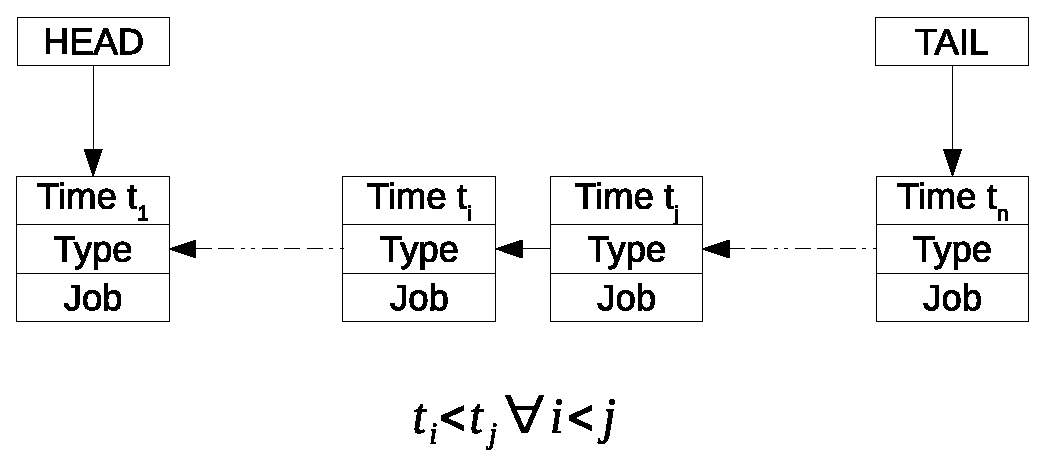
\includegraphics[width=0.7\textwidth]{figures/eventq}
\caption{Coda prioritaria di eventi, ordinata per istante di scadenza}
\label{eventq}
\end{figure}
%
\\Un generico evento è composto dai seguenti campi:
\begin{itemize}
\item L’istante in cui l’evento si verifica
\item La tipologia di evento (arrivo, partenza, setup)
\item Il job associato
\item Un array contenente lo stato del sistema (la sua struttura verrà discussa
più avanti)
\end{itemize}
%
Ogniqualvolta viene creato un evento, questo viene inserito nella coda nella
posizione opportuna tramite un’operazione di \emph{enqueue}, affinché ogni 
operazione di \emph{dequeue} estragga l’evento più imminente.

Il tempo di simulazione è regolato da un clock virtuale che tiene conto
dell’istante corrente e del successivo in modo tale da poter considerare
intervalli di tempo utili per il calcolo di statistiche di tipo time-averaged.

\begin{figure}[!h]
\begin{lstlisting}[title=Impementazione Evento e Clock Virtuale (basic.h)]
struct event {
    double time;
    struct job_t job;
    unsigned int type;
    unsigned int n[4];
};

typedef struct {           /* simulation clock                  */
    double current;        /*   current time                    */
    double next;           /*   next (most imminent) event time */
} clock;
\end{lstlisting}
\end{figure}

%
\subsubsection{Variabili di Output}
I dati che man mano devono essere raccolti durante la simulazione sono
memorizzati in variabili suddivise in base alla tipologia e al nodo di
esecuzione dei job. Per esempio, lo stato del sistema, così come il numero di
arrivi e completamenti, è implementato tramite un array di dimensione 4, di cui
ogni slot corrisponde ad una combinazione classe-nodo a cui il job può essere
associato. 

L’accesso ad uno slot dell’array viene effettuato tramite un indice
che viene calcolato tramite la somma di macro che rappresentano le varie
combinazioni, infatti, se si vuole considerare il numero di job di classe 1 in
esecuzione nel cloud basta accedere all’array tramite l’indice che deriva dalla
somma delle macro J\_CLASS1 e CLOUD ($0 + 2 = 2$). La tabella~\ref{comb}
descrive le possibili combinazioni di macro legate all’indice di accesso.
\begin{table}[!h]
\begin{tabular}{c|c|c|c}
          & CLET & CLOUD & SETUP \\
\hline
J\_CLASS1 & 0    & 2     &       \\
\hline
J\_CLASS2 & 1    & 3     & 4     \\
\end{tabular}
\centering
\caption{Combinazioni per il calcolo dell'indice degli array}
\label{comb}
\end{table}
%
\begin{figure}[!h]
\begin{lstlisting}[title=Definizione macro Nodi e Classi (basic.h)]
 #define J_CLASS1    0           /* job class type 1 */
 #define J_CLASS2    1           /* job class type 2 */
 #define CLET        0           /* cloudlet index   */
 #define CLOUD       2           /* cloud index      */
 #define SETUP       3           /* setup index      */
\end{lstlisting}
\end{figure}
\subsubsection{Task}
Un generico task, anche detto job, viene implementato come una struttura
specifica dotata dei seguenti attributi: 
\begin{itemize}
\item[id]: identificatore univoco necessario ad effettuare un riordino dei job
nel momento in cui vanno considerate le statistiche in un ordine corrispondente
agli istanti di arrivo dei singoli job
\item[class]: specifica la classe del job, può assumere il valori J\_CLASS1 e
J\_CLASS2 (macro definite nel file di configurazione); 
\item[node]: specifica il nodo in cui il job è in esecuzione, può assumere i
valori CLET, CLOUD, SETUP (macro definite nel file di configurazione), che
corrispondono rispettivamente a cloudlet, cloud e nodo di setup; 
\item[service]: array che memorizza i tempi di risposta seguendo la stessa regola
delle combinazioni che riguarda anche lo stato del sistema. Un job di classe 1
in esecuzione nel cloud avrà un tempo di risposta non nullo nello slot relativo,
un job interrotto avrà un tempo di risposta non nullo sia nello slot riguardante
il nodo cloudlet che in quello riguardante il nodo cloud. 
\item[setup]: tempo che un job trascorre in fase di setup. Il valore rimane
nullo nel caso in cui il job non viene interrotto.  
%
\end{itemize}
\begin{figure}[!h]
\begin{lstlisting}[title=basic.h]
struct job_t {
    unsigned long id;
    unsigned int class;
    unsigned int node;
    double service[4];
    double setup;
};
\end{lstlisting}
\end{figure}
%
%
\subsection{Generazione dell'input}
I dati di input della simulazione, corrispondenti ai tempi di interarrivo e di
servizio dei singoli job, vengono generati a runtime in base alle informazioni
note sulle rispettive distribuzioni esponenziali. Per ottenere tali
distribuzioni sono state utilizzate le funzioni delle librerie \emph{rvgs} e
\emph{rngs} di \emph{Steve Park} e \emph{Dave Geyer} descritte in \cite{leemis}.

La funzione \emph{GetArrival()}, ogniqualvolta viene chiamata, restituisce il
più imminente istante di arrivo tra un job di classe 1 ed uno di classe 2 e
memorizza nella variabile $j$, passata per riferimento, la classe del job in
questione. Tali istanti di arrivo vengono calcolati progressivamente a seguito
della generazione dei tempi di interarrivo tra un job e l’altro, più
precisamente, non appena viene restituito un istante di arrivo relativo al job
di una classe, viene calcolato il successivo per la medesima classe.

La funzione \emph{GetService()} restituisce un valore che deriva dalla
generazione di un tempo di servizio esponenziale con media stabilita in base ai
parametri $j$ e $n$ passati come argomento che indicano rispettivamente la
classe ed il nodo di esecuzione del job.

La funzione \emph{GetSetup()} restituisce semplicemente un valore generato a
partire da una distribuzione esponenziale di media $E[S_{setup}]$.

Le funzioni in questione sono elencate di seguito. Si noti che prima di ogni
chiamata alle funzioni della libreria \emph{rvgs} viene selezionato, tramite la
funzione \emph{SelectStream()}, un flusso di generazione di numeri
pseudo-casuali distinto, affinché sia garantita il più possibile l’indipendenza
tra le sequenze di numeri generate.  
%
\begin{figure}[!h]
\begin{lstlisting}[title=basic.h]
double GetArrival(unsigned int *j)
{
    const double mean[2] = {1/L1, 1/L2};
    static double arrival[2] = {START, START};
    static int init = 1;
    double temp;

    if (init) {
        SelectStream(0);
        arrival[0] += Exponential(mean[0]);
        SelectStream(1);
        arrival[1] += Exponential(mean[1]);
        init=0;
    }

    if (arrival[0] <= arrival[1])
        *j = 0;
    else
        *j = 1;

    temp = arrival[*j];
    SelectStream(*j);
    arrival[*j] += Exponential(mean[*j]);
 
    return temp;
}              
             
double GetService(int j, int n)
{                            
    const double mean[4] = {1/M1CLET, 1/M2CLET,
                            1/M1CLOUD, 1/M2CLOUD, 
                            1/MSETUP};
    SelectStream(j + n + 2);               
    return Exponential(mean[j + n]);      
}                                       
\end{lstlisting}
\end{figure}
%
%
\subsection{Flusso principale}
Il programma che si occupa dell’esecuzione della simulazione è contenuto nel
file \emph{cloudq.c}. Il flusso di esecuzione principale consiste nell’eseguire
le varie replicazioni della simulazione producendo, per ognuna di esse, dei file
di output che vengono presi in input da altri programmi che si occupano di
elaborare i dati, tali programmi sono denominati \emph{bm\_*.c} e producono, per
ogni replicazione e per ogni metrica, un campione di $k$ medie di batch di
dimensione $b$ sul quale viene calcolato un intervallo di confidenza del $95\%$.
\\Ogni replicazione della simulazione è composta dalle seguenti fasi:
%
\begin{enumerate}
\item Inizializzazione: apertura dei file di output, reset delle variabili (e
del clock virtuale?), settaggio del seme per il PRNG, generazione ed inserimento
nella coda del primo evento di arrivo.

\item Processamento degli eventi: fintanto che la coda degli eventi non è vuota,
viene aggiornata l’area relativa alla popolazione nel tempo di simulazione
corrente, viene estratto l’evento in cima alla coda ed a seconda del tipo di
evento si attuano le azioni descritte nell’algoritmo~\ref{alg};

\item Terminazione: chiusura dei file di output e stampa su schermo dei
risultati della replicazione.

\end{enumerate}
%
\begin{figure}[!h]
\begin{lstlisting}[title=cloudq.c]
/* initialize data structures */
/* ..... */

while (queue.head != NULL) { 

    e = dequeue_event(&queue);
    t.next = e->time;                     /* next event time   */

    for (i = 0; i < 5; i++)               /* update integral   */
        area[i] += (t.next - t.current) * n[i];

    t.current = t.next;                   /* advance the clock */

    switch (e->type) {
    case E_ARRIVL:              
        /* process an arrival */
        /* ..... */
    case E_SETUP:
        /* process an arrival */
        /* ..... */
    case E_DEPART: 
        /* process a departure */
        /* ..... */
        /* write data to outfile */
        /* ..... */
    default:
        handle_error("unknown event type");
    }
}

/* ..... */
\end{lstlisting}
\end{figure}
%
\subsubsection{Gestione degli eventi}
A livello computazionale, le operazioni che corrispondono ai vari eventi
(indicati con le macro specificate nel file basic.h) sono le seguenti:
\begin{itemize}
\item[E\_ARRIVL]: evento di arrivo, a seconda della classe del job e dello stato
del sistema, vengono aggiornate le variabili degli arrivi e quelle della
popolazione corrente, tramite la funzione \emph{srvjob()} viene creato e
inserito nella coda un evento di partenza dal nodo in cui il job va
concettualmente in esecuzione, per un tempo di servizio che viene generato
tramite la funzione \emph{GetService()} e memorizzato nell’apposita variabile
del job. Se si verificano le condizioni per cui avviene l’interruzione di un
job, tramite la funzione \emph{rplcjob()} viene rimosso un evento di partenza
relativo ad un job di classe 2 in esecuzione sul cloudlet, viene creato un
evento di setup a cui viene associato il nodo rimosso con un nuovo tempo di
servizio generato dalla funzione \emph{GetService()}, infine viene creato ed
immesso nella coda un evento di partenza dal cloudlet con associato il nuovo job
appena arrivato.\\
Una volta che un evento di arrivo viene processato, viene generato il successivo
ed inserito nella coda. Si può osservare che, ad ogni istante, nella coda è
presente un solo evento di arrivo, poiché un evento di tale tipo viene generato
soltanto dopo che il precedente viene processato.

\item[E\_DEPART]: evento di partenza, vengono aggiornate le variabili relative
alla popolazione del sistema ed ai completamenti in base alla classe del job e
al nodo di servizio, inoltre vengono scritti i dati correnti sui file di output,
quindi, una metrica di interesse, viene registrata ad ogni completamento di un
job, anche quelle non relative ai singoli job come la popolazione media.

\item[E\_SETUP]: evento di setup, indica la terminazione della fase di setup di
un job interrotto, viene generato un nuovo evento di partenza dal cloud e viene
aggiornato lo stato della popolazione del sistema.

\item[E\_IGNRVL]:
\end{itemize}

[CODICE RELATIVO AI VARI EVENTI]

%
\begin{figure}[!h]
\begin{lstlisting}[title=cloudq.c]

double srvjob(struct job_t job, unsigned int node,
                struct queue_t *queue, clock t)
{
    double service = GetService(job.class, node);
    struct event *e = alloc_event();
    memset(e, 0, sizeof(struct event));

    job.node = node;
    job.service[job.class + node] = service;
    e->job = job;
    e->time = t.current + service;
    e->type = E_DEPART;
    enqueue_event(e, queue);

    return service;
}


/* return the cloudlet execution time of the removed job */
double rplcjob(struct queue_t *queue, clock t, unsigned int n)
{
    double service;
    double left;                      // remaining service time
    double setup = GetService(J_CLASS2 + SETUP);
    struct event *temp = alloc_event();
    struct job_t *job = &temp->job;
    struct event *e = NULL;
    
    job->class = J_CLASS2;
    job->node = CLET;
    temp->type = E_DEPART;
    e = remove_event(queue, temp, rmpos(n));
    
    left = e->time - t.current;     

    e->time = t.current + setup;
    e->type = E_SETUP;

    job = &e->job;
    job->node = SETUP;
    job->service[J_CLASS2 + SETUP] = setup;
    service = job->service[J_CLASS2 + CLET];
    job->service[J_CLASS2 + CLET] -= left;

    enqueue_event(e, queue);
    free(temp);

    return service - left;
}
\end{lstlisting}
\end{figure}
%
%
\subsection{Produzione ed Elaborazione dell'Output}
La simulazione viene eseguita un numero $R$ di volte in modo da ottenere un
campione di tale dimensione con cui generare un intervallo di confidenza al 95\%
per le statistiche ottenute.  Le replicazioni della simulazione sono gestite con
un ciclo for all’inizio del quale vengono re-inizializzate tutte le variabili e
viene reimpostato il seme per il PRNG affinché le distribuzioni generate in ogni
replicazione siano indipendenti. In ogni replicazione i valori delle variabili
vengono scritti in modo iterativo su dei file di output che vengono poi
elaborati tramite un successivo programma (\emph{bm\_*.c}) per il calcolo delle
metriche di interesse.
\subsubsection{Tempo di Servizio} 
Il file \emph{service.dat} contiene le informazioni riguardanti i tempi di
servizio di ogni job in base alla sua classe ed al nodo su cui è stato eseguito:
ogni riga corrisponde ad un singolo job tranne la prima in cui sono presenti i
completamenti sempre suddivisi per combinazione classe-nodo, necessari al
calcolo della grandezza dei batch. Infatti se durante la simulazione sono stati
processati $c_1$ job di classe 1 ed $c_2$ job di classe 2, la dimensione dei
relativi batch sarà rispettivamente $c_1/K$ e $c_2/K$, con $K$ pari al numero di
batch del campione.

Poiché i tempi di servizio vengono scritti ad ogni completamento dei job, quindi
in un ordine che non corrisponde a quello di arrivo, è necessario riordinare le
righe del file, questo viene fatto tramite la chiamata di sistema
\emph{system()}, che permette di eseguire il comando shell per il riordino delle
righe, a tale scopo viene inserito l’id del job (assegnato in ordine di arrivo)
all’inizio di ogni riga.

[CODICE SCRITTURA SU FILE E RIORDINO]

[FIGURA FILE DI OUTPUT]

Il programma \emph{bm\_srv} si occupa dell’elaborazione di questo file, leggendo
riga per riga e riempiendo le apposite variabili, distinguendo la tipologia del
job ed il nodo di esecuzione in base ai valori non nulli della riga.

Ogni metrica è implementata con un array di $K$ elementi, i quali vengono
popolati sommando esattamente $b$ valori della metrica che compongono un batch.
Al termine del ciclo di processamento delle righe, ogni elemento viene diviso
per $b$ per calcolare il valor medio.

In questo modo l’array costituisce un campione di dimensione $K$ per la metrica,
per il quale il programma calcola un intervallo di confidenza con un livello di
significatività pari a $\alpha = 0.05$.

[CODICE bm\_srv.c]
%
\subsubsection{Throughput, popolazione, e percentuale di interruzioni}
I file \emph{throughput.dat}, \emph{population.dat} e \emph{interruption.dat}
contengono valori relativi rispettivamente al throughput, alla popolazione media
e alla percentuale di job interrotti.

Anche se sono metriche che non si riferiscono direttamente ad un job, è stato
comunque scelto l’evento di completamento come istante di campionamento, in modo
da avere conformità tra tutti i file di output e controllo sul numero di valori
che vengono raccolti, poiché il programma raccoglie una quantità di dati pari al
numero di job che devono essere processati durante la simulazione.

I file vengono progressivamente generati, come per il file \emph{service.dat},
scrivendo su ogni riga i valori corrispondenti alla combinazione classe-nodo.

L’elaborazione differisce invece perché ogni riga contribuisce al popolamento
degli array, quindi ognuno di questi avrà i batch della stessa dimensione pari
al rapporto tra il numero di righe N\_JOBS e la dimensione del campione $K$.

[CODICE ED ESEMPIO DI OUTPUT]

[CODICE bm\_thr.c]
%

%
%
